\section*{Question 4}
Here, I replicated all the results from the previous question by implementing three changes in the data:
\begin{itemize}
    \item I create 10 portfolios based on the characteristic of the stocks.
    \item I exclude the stocks with a price lower than 5 dollars.
    \item I exclude the stocks with a market capitalization lower than 20 percentiles of the market capitalization each month.
\end{itemize}

\begin{enumerate}[(a)]
    \setcounter{enumi}{2}
\item 
The cumulative return of long-short portfolio is shown in the figure \ref{fig:4c}. The pattern is quiet similar to the previous question. The cumulative return for equal weighted is higher that value weighted. 

\begin{figure}
    \centering
    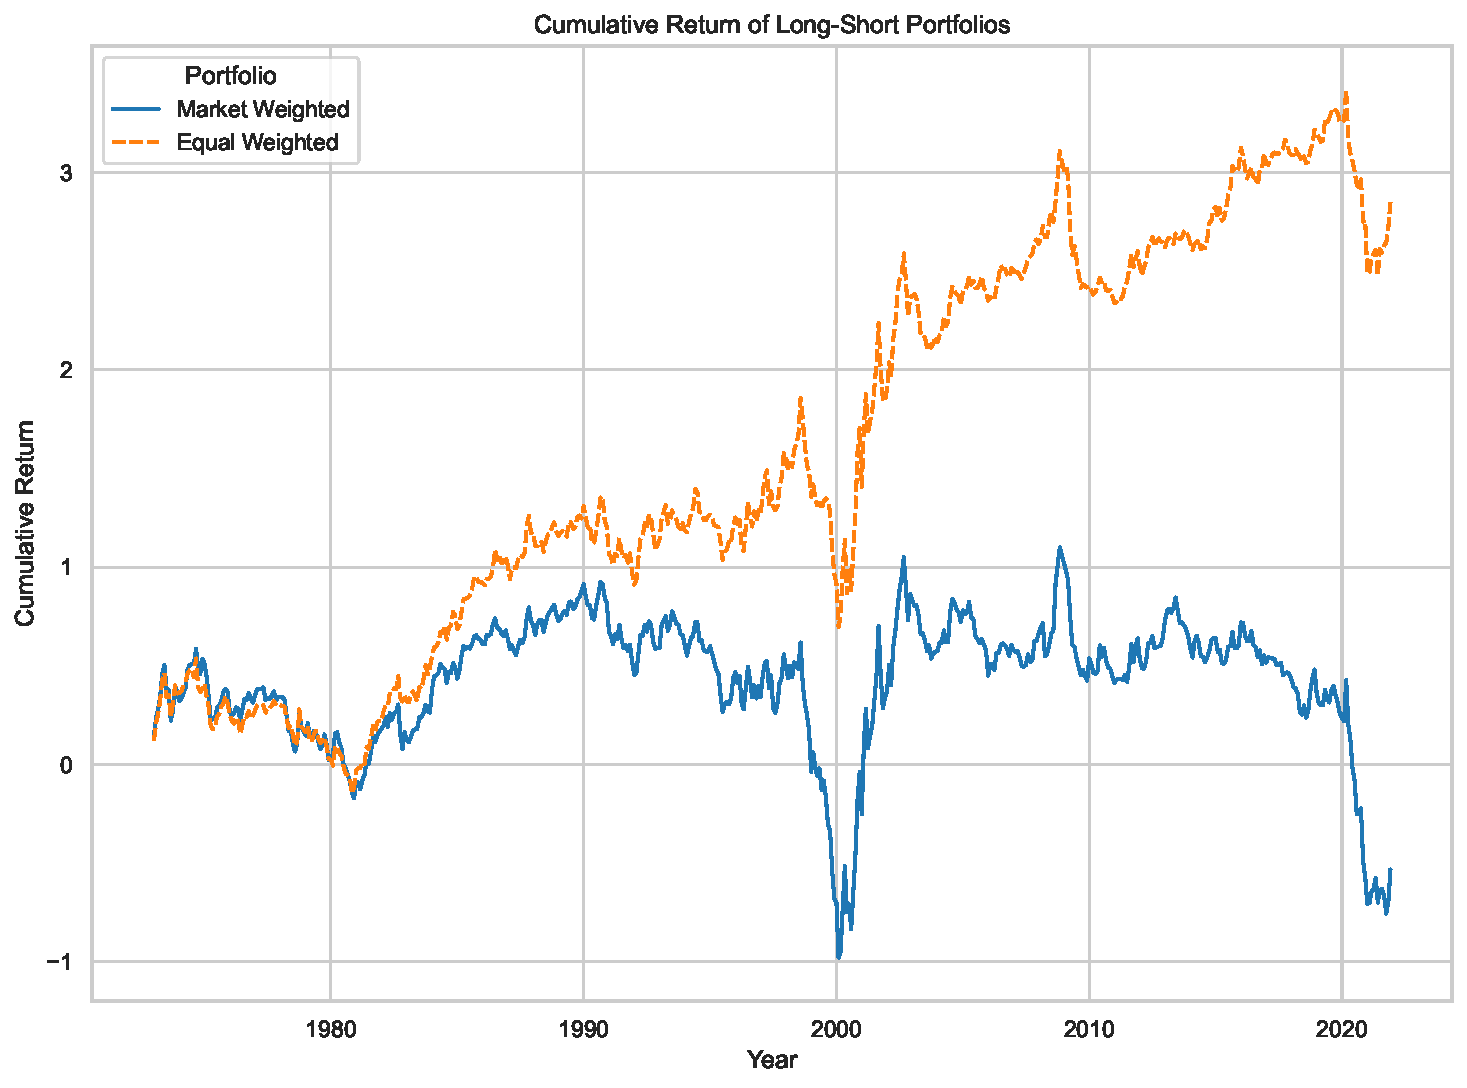
\includegraphics[width=0.6\textwidth]{Out/4_3.pdf}
    \caption{Time series of the average returns of the long-short portfolio.}
    \label{fig:4c}
\end{figure}

Now you can see the $\alpha$ test for long-short portfolio with different models in the table \ref{tab:4c}. The results are in line with the previous question but the statistical significance is lower.

\begin{table}[htbp]
    \caption{$\alpha$ test for long-short portfolio with different models}
    \begin{tabularx}{\linewidth}{CC}
        \caption*{Equal Weighted }
        \begin{tabular}{lcc}
\toprule
 & $\alpha$ & $Pvalue$ \\
\midrule
CAPM & 0.011 & 0.000 \\
FF3 & 0.008 & 0.000 \\
CAR & 0.005 & 0.005 \\
FF5 & 0.004 & 0.025 \\
HXZ & 0.002 & 0.245 \\
\bottomrule
\end{tabular}

        &
        \caption*{Market Weighted }
        \begin{tabular}{lcc}
\toprule
 & $\alpha$ & $Pvalue$ \\
\midrule
CAPM & 0.005 & 0.040 \\
FF3 & 0.003 & 0.170 \\
CAR & 0.000 & 0.825 \\
FF5 & -0.002 & 0.221 \\
HXZ & -0.004 & 0.103 \\
\bottomrule
\end{tabular}

    \end{tabularx}
\end{table}
\item Here are the results for the $\alpha$ test for long-short portfolio for in and out of sample with equal weighting and market weighting in the tables \ref{tab:4d1} and \ref{tab:4d2} respectively. 

\begin{table}[htbp]
    \caption{$\alpha$ test long-short portfolio for in and out of sample with equal weighting}
    \begin{tabularx}{\linewidth}{CC}
        \caption*{Sample period }
        \begin{tabular}{lcc}
\toprule
{} &  \$\textbackslash alpha\$ &  \$Pvalue\$ \\
\midrule
CAPM &     0.011 &     0.000 \\
FF3  &     0.007 &     0.002 \\
CAR  &     0.005 &     0.023 \\
FF5  &     0.004 &     0.107 \\
HXZ  &     0.004 &     0.141 \\
\bottomrule
\end{tabular}

        &
        \caption*{Post-publication period}
        \begin{tabular}{lcc}
\toprule
 & $\alpha$ & $Pvalue$ \\
\midrule
CAPM & 0.014 & 0.000 \\
FF3 & 0.013 & 0.000 \\
CAR & 0.010 & 0.000 \\
FF5 & 0.007 & 0.002 \\
HXZ & 0.004 & 0.077 \\
\bottomrule
\end{tabular}

    \end{tabularx}
\end{table}

\begin{table}[htbp]
    \caption{$\alpha$ test long-short portfolio for in and out of sample with market weighting}
    \begin{tabularx}{\linewidth}{CC}
        \caption*{Sample period }
        \begin{tabular}{lcc}
\toprule
{} &  \$\textbackslash alpha\$ &  \$Pvalue\$ \\
\midrule
CAPM &     0.007 &     0.009 \\
FF3  &     0.003 &     0.112 \\
CAR  &     0.002 &     0.493 \\
FF5  &     0.001 &     0.746 \\
HXZ  &     0.002 &     0.596 \\
\bottomrule
\end{tabular}

        &
        \caption*{Post-publication period}
        \begin{tabular}{lcc}
\toprule
 & $\alpha$ & $Pvalue$ \\
\midrule
CAPM & 0.007 & 0.117 \\
FF3 & 0.006 & 0.058 \\
CAR & 0.004 & 0.207 \\
FF5 & -0.000 & 0.877 \\
HXZ & -0.003 & 0.373 \\
\bottomrule
\end{tabular}

    \end{tabularx}
\end{table}


\end{enumerate}